\documentclass[tikz,border=4pt]{standalone}
\usepackage{amsmath}
\begin{document}
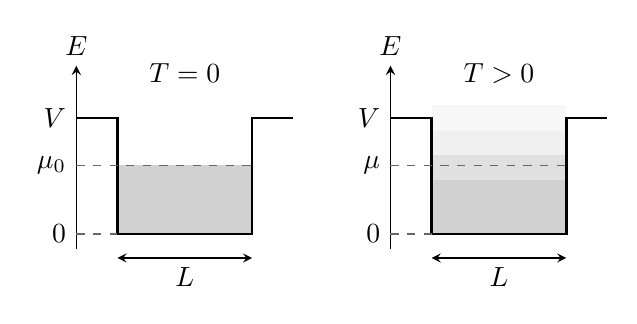
\begin{tikzpicture}[>=stealth, thick, scale=0.95]
  % Left: T = 0
  \begin{scope}[xshift=-2.4cm]
    % Shaded occupied states 0 to mu0
    \fill[black!18] (0.55, 0) rectangle (2.35, 0.92);

    % Potential box
    \draw[line width=0.95pt] (0, 1.55) -- (0.55, 1.55) -- (0.55, 0) -- (2.35, 0) -- (2.35, 1.55) -- (2.9, 1.55);

    % Energy axis
    \draw[->, line width=0.5pt] (0, -0.2) -- (0, 2.25) node[above] {$E$};
    \node[left] at (0, 0) {$0$};
    \node[left] at (0, 0.92) {$\mu_0$};
    \node[left] at (0, 1.55) {$V$};

    % Guide dashed lines
    \draw[dashed, line width=0.45pt, black!60] (0, 0) -- (0.55, 0);
    \draw[dashed, line width=0.45pt, black!60] (0, 0.92) -- (2.35, 0.92);

    % Width L
    \draw[<->, line width=0.45pt] (0.55, -0.32) -- (2.35, -0.32) node[midway, below] {$L$};

    \node at (1.45, 2.15) {$T = 0$};
  \end{scope}

  % Right: T > 0
  \begin{scope}[xshift=1.8cm]
    % Occupied states with thermal smearing around mu
    \fill[black!18] (0.55, 0) rectangle (2.35, 0.72);
    \fill[black!12] (0.55, 0.72) rectangle (2.35, 1.05);
    \fill[black!6] (0.55, 1.05) rectangle (2.35, 1.38);
    \fill[black!3] (0.55, 1.38) rectangle (2.35, 1.72);

    % Potential box
    \draw[line width=0.95pt] (0, 1.55) -- (0.55, 1.55) -- (0.55, 0) -- (2.35, 0) -- (2.35, 1.55) -- (2.9, 1.55);

    % Energy axis
    \draw[->, line width=0.5pt] (0, -0.2) -- (0, 2.25) node[above] {$E$};
    \node[left] at (0, 0) {$0$};
    \node[left] at (0, 0.92) {$\mu$};
    \node[left] at (0, 1.55) {$V$};

    % Guide dashed lines
    \draw[dashed, line width=0.45pt, black!60] (0, 0) -- (0.55, 0);
    \draw[dashed, line width=0.45pt, black!60] (0, 0.92) -- (2.35, 0.92);

    % Width L
    \draw[<->, line width=0.45pt] (0.55, -0.32) -- (2.35, -0.32) node[midway, below] {$L$};

    \node at (1.45, 2.15) {$T > 0$};
  \end{scope}
\end{tikzpicture}
\end{document}
